\documentclass[mathserif, blue]{beamer}%Agregar ,notes antes del ] para incluir las notas.
%~ \documentclass[handout]{beamer}
% Paquetes usados
\usepackage[utf8]{inputenc}
\usepackage[spanish, es-tabla]{babel}
\usepackage{indentfirst}
\usepackage{beamerthemeshadow}
\usepackage{xspace}
\usepackage{latexsym}
\usepackage{ulem}

\newcommand{\tab}[1]{\hspace{.12\textwidth}\rlap{#1}}

\parskip=1ex

\title{Recolección online de grabaciones para el estudio de las variantes argentinas del español}
\author{Fernando Bugni}
\institute{Departamento de Computación - FCEyN - UBA}
\date{Fecha}

\begin{document}
	
\title{Recolección online de grabaciones para el estudio de las variantes argentinas del español}
\author{Fernando Bugni}
\institute{Departamento de Computación - Facultad de Ciencias Exactas - \\Universidad de Buenos Aires}
\date{2014}

\frame{\titlepage}

% % % % Introducción

\section{Introducción}
\begin{frame}
	\frametitle{Variantes del español en Argentina}
	\begin{figure}
		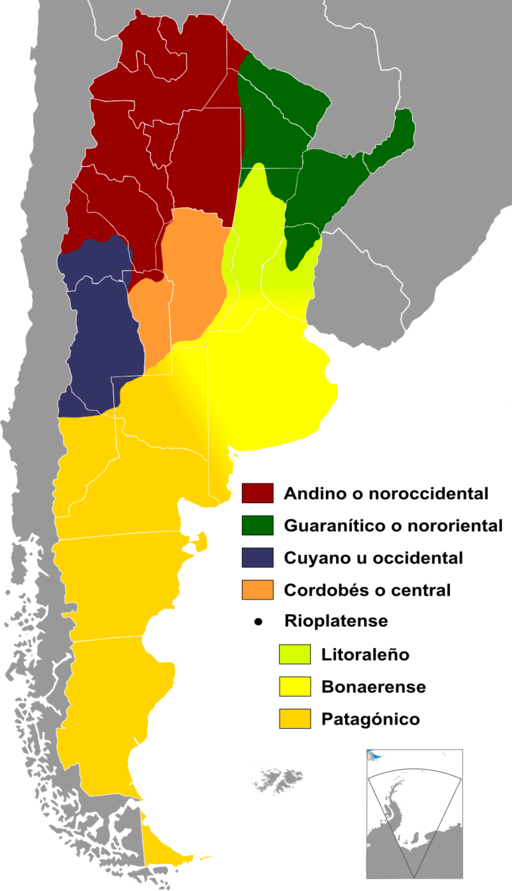
\includegraphics[scale=0.3]{../template_tesis/Images/Dialectos_del_idioma_espanol_en_Argentina.png}\\
	\end{figure}
\end{frame}

\begin{frame}
	\frametitle{Diferencias entre Córdoba y Buenos Aires}
	\begin{itemize}\itemsep=3ex
		\item \textbf{Los hablantes de Córdoba estiran la sílaba anterior a la acentuada mientras los de Buenos Aires no realizan esto} \\ 
	\end{itemize}	
	
	\begin{center}
		\textit{`Especta\textcolor{red}{\textbf{\textit{cu}}}\textcolor{blue}{lar}'}
	\end{center} 
	
	\tab{Sílaba acentuada en \textcolor{blue}{\textit{`-lar'}}} \\ 
	\tab{La sílaba anterior \textcolor{red}{\textit{`-cu-'}} se alarga para hablantes de Córdoba}
\end{frame}

\begin{frame}
	\frametitle{Diferencias entre Córdoba y Buenos Aires}
	\begin{itemize}\itemsep=3ex
		\item \textbf{Los hablantes de Córdoba aspiran y elisionan la /s/ al finalizar una palabra. Esto no sucede para Buenos Aires} \\ 
	\end{itemize}	
	
	\begin{center}
		\textit{`Pájaro\textcolor{red}{\textbf{\textit{s}}}'}
	\end{center} 
	
	\begin{center}
		/\textcolor{red}{\textbf{\textit{s}}}/ se acorta su duración en el hablante de Córdoba
	\end{center}
\end{frame}

\begin{frame}
 	\frametitle{Diferencias entre Córdoba y Buenos Aires}
 	\begin{itemize}\itemsep=3ex
 		\item \textbf{Para hablantes de Córdoba, la /s/ antes de la /c/ o /t/ suenan más suaves que para hablantes de Buenos Aires} \\ 
 	\end{itemize}
 	
 	\begin{center}
 		\textit{`Mo\textcolor{red}{s}ca'}
 	\end{center} 
 	
 	\begin{center}
 		/\textcolor{red}{s}/ suena más suave para Córdoba que para Buenos Aires
 	\end{center}
\end{frame}
 
\begin{frame}
 	\frametitle{Diferencias entre Córdoba y Buenos Aires}
 	\begin{itemize}\itemsep=3ex
 		\item \textbf{La `c' antes de la `t' se pronuncia con menor frecuencia para hablantes de Córdoba que para hablantes de Buenos Aires} \\ 
 	\end{itemize}
 	
 	\begin{center}
 		\textit{`Do\textcolor{red}{c}tor'}
 	\end{center} 
 	
 	\begin{center}
 		No debe sonar el fonema /\textcolor{red}{c}/
 	\end{center}
\end{frame}
 
\begin{frame}
	\frametitle{Diferencias entre Córdoba y Buenos Aires}
	\begin{itemize}\itemsep=3ex
		\item \textbf{En hablantes cordobeces la /r/ no vibra mientras que en Buenos Aires pasa lo contrario} \\ 
	\end{itemize}	
	
	\begin{center}
		\textit{`Espá\textcolor{red}{rr}ago'}
	\end{center} 
	
	\begin{center}
		Para Córdoba /\textcolor{red}{r}/ debe ser suave en comparación de Buenos Aires
	\end{center}
\end{frame} 

% % % % Diseño del experimento
\begin{frame}
	\frametitle{Diseño del experimento}
	\begin{itemize}\itemsep=10ex
		\item \textbf{Frases Comúnes}: habla espontánea
		\item \textbf{Frases Amper}: reconocer palabra acentuada
	\end{itemize}	
\end{frame} 

\begin{frame}
	\frametitle{Diseño del experimento}
	{\Large Frases Comúnes} \\
	Pronunciar frases popularmente conocidas
	
	\begin{itemize}
		\item Objetivo: pronunciación espontánea
		\item Regla a cubrir: 
	\end{itemize}
\end{frame} 

\begin{frame}
	\frametitle{Diseño del experimento}
	\begin{center}
		\textbf{`En la pelea se conoce al soldado,} \\ 
		\textbf{sólo en la \textcolor{red}{victoria} se conoce al \textcolor{red}{caballero}’}
	\end{center}
	
	\begin{itemize}
		\item \textcolor{red}{\textbf{`victoria’}} cubre la regla 4 que nos propone medir la duración de la \textit{/c/} antes de la \textit{/t/}. 
		\item \textcolor{red}{\textbf{`caballero’}} para la regla 5: el fonema \textit{/ll/} se pasa a \textit{/i/} 
	\end{itemize}	
\end{frame} 

\begin{frame}
\frametitle{Diseño del experimento}
	{\Large Frases Amper} \\
	Pronunciar frases con una estructura fija variando acentuaciones
	
	\begin{itemize}
		\item Objetivo: cubrir acentuaciones
		\item Regla a cubrir: estiramiento de la sílaba anterior a la acentuada
	\end{itemize}
	
{\footnotesize 	
	\begin{center}
		\textit{Sujeto+`` salió ’’+Adjetivo} 
	
		\begin{itemize}
			\item Sujeto: \textit{``El canapé’’, ``El repollo’’, ``El espárrago’’}.
			\item Adjetivo: \textit{``espectacular’’, ``delicioso’’, ``riquísimo’’}.
		\end{itemize}
		
	\end{center}
}
\end{frame} 

\begin{frame}
	\frametitle{Diseño del experimento}

	\begin{center}
		\textbf{``El canapé salió delicioso’’}
	\end{center}
	
	\begin{itemize}
		\item Canapé: palabra aguda
		\item Delicioso: palabra grave
	\end{itemize}
\end{frame} 

\begin{frame}
	\frametitle{Diseño del experimento}
	
	Trazas: combinación de frases
	
\end{frame}

\begin{frame}
\frametitle{Compuertas - AND}
\begin{figure}
\begin{tabular}{cc|c}
A & B & A AND B \\
\hline
0 & 0 & 0\\
0 & 1 & 0\\
1 & 0 & 0\\
1 & 1 & 1
\end{tabular}
\end{figure}
\end{frame}

% % %


\end{document}

%
%\begin{frame}
%	\frametitle{Compuertas - datasheet}
%	\begin{figure}
%		\includegraphics[scale=0.4]{datasheetDM7408N.png}\\
%	\end{figure}
%\end{frame}

%\begin{frame}
%	\frametitle{Propiedades}
%	\begin{center}
%	\begin{footnotesize}
%	\begin{tabular}[h]{|c|c|c|}
%	\hline
%	Identidad & $1.A=A$                      &     $0+A=A$            \\
%	 Nulo            &      $0.A=0$                      &     $1+A=1$            \\
%	 Idempotencia    &       $A.A=A$                      &     $A+A=A$            \\      
%	 Inverso         &       $A.\overline{A}=0$           &     $A+\overline{A}=1$ \\      
%	 Conmutatividad  &       $A.B=B.A$                    &     $A+B=B+A$          \\
%	 Asociatividad   &       $(A.B).C=A.(B.C)$            &     $(A+B)+C=A+(B+C)$  \\
%	 Distributividad &      $A+(B.C) = (A+B).(A+C)$      &     $A.(B+C)=A.B+A.C$  \\
%	 Absorci\'on     &       $A.(A+B)=A$                  &     $A+A.B = A$        \\
%	 De Morgan       &  $\overline{A.B} = \overline{A} + \overline{B}$ & $\overline{A+B} = \overline{A} . \overline{B}$ \\
%	\hline
%	\end{tabular}\\
%	\end{footnotesize}
%	\end{center}
%\end{frame}


%\begin{frame}
%\frametitle{M\'as circuitos combinatorios!}
%\pause			
%\underline{Decodificador de n bits:} Tiene n entradas y $2^n$ salidas. Sea k el n\'umero representado en binario en la entrada del decodificador, la salida $e_k$ tendr\'a un uno l\'ogico, mientras que para todas las dem\'as se\~nales de salida habr\'a un cero l\'ogico.\\
%\pause
%\underline{Codificador de n bits:} Tiene n entradas y $log_2(n)$ salidas. En la salida muestra en binario el n\'umero de la entrada que esta levantada, de haber mas de una o ninguna, el comportamiento del circuito depender\'a de la implementaci\'on del fabricante.\\
%\pause
%\underline{Multiplexor de n entradas:} Tienen n entradas, una salida y $log_2(n)$ se\~nales de control. Mediante las se\~nales de control se indica cual entrada es requerida en la salida.\\
%\pause
%\underline{Demultiplexor de n salidas:} Tienen n salidas, una entrada y $log_2(n)$ se\~nales de control. Igual que el multiplexor, pero elijo mediante las se\~nales de control por cual se\~nal de salida muestro la entrada.
%\end{frame}
%
%\begin{frame}
%\frametitle{La práctica...}
%\begin{center}
%Con lo visto hoy pueden realizar hasta\\ el ejercicio 13 de la práctica 2.
%
%Bibliograf\'ia recomendada: The Essentials of Computer Organization and Architecture - Linda Null
%- Cap\'itulo 3
%\end{center}
%\end{frame}